\subsection{Introduction to Sound}
Soundscape ecologists use the mathematics of waves in order to derive meaning from sound. This section provides a background on our understanding of sound, including the basics of waves, representation of waves, and Laplace transforms.

\subsubsection{What is Sound?}
The simplest form of sound that one can listen to is a tone. But what does it mean for us to hear a tone? We must start with what hearing is and what it means for humans to pick up sound.\par
It all starts with compressions in the air. As physical objects move within our environment, they compress air around them. This compression travels through the gaseous environment we live in. This chain reaction continues the compression in the form of sound waves. When these waves arrive to a listener, whether that be a human or a microphone, it can pick up on these fluctuations in the pressure of the air around it. This change in air pressure is what we call sound.
\begin{center}
  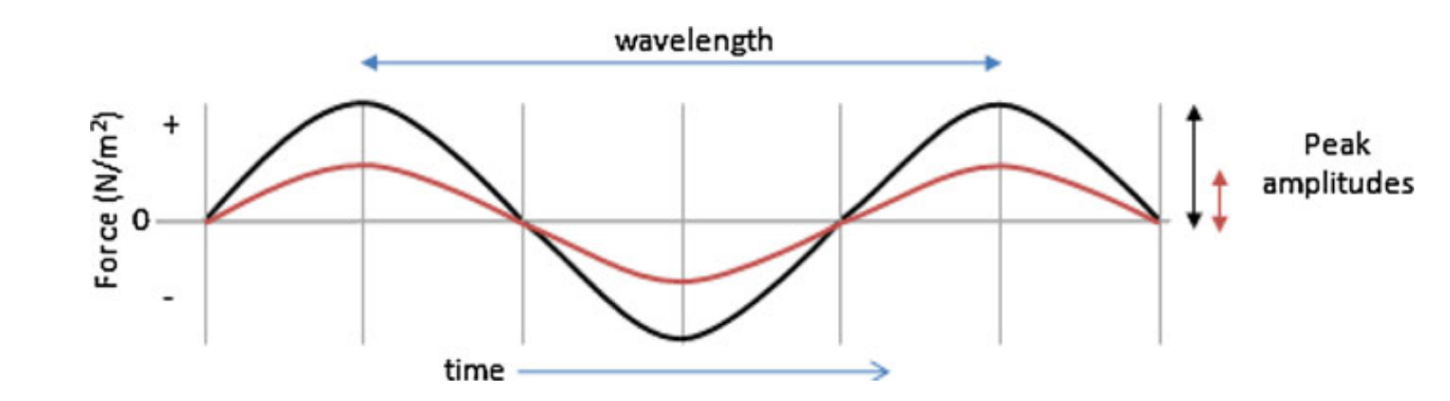
\includegraphics[width=0.85\textwidth]{wave} \\[12pt]
\end{center}
\cite{villanueva}
When we take a closer look at waves, certain similarities amongst all waves start to appear. These characteristics can be used to describe waves and how they interact with their environment. The most prominent feature is that simple tones are comprised of simple sinusoidal waves. These are generally graphed as the force of pressure over time. Once graphed, the wavelength of a wave can be measured. This measurement shows the distance between the peak forces over time. One wavelength can be understood as one cycle of the wave. The amount of cycles that appear per time unit can be described as the frequency of the wave. A higher frequency wave correlates to a higher ``pitch'' when heard. Another correlation between these graphed waves and sound is the height of wave peaks. The higher the wave peak, the louder the sound is. The ``loudness'' of a sound is measures in decibels (dB), which are measured in base 10 units. This measurement system is a reference system, with 0 being the minimum value that a healthy human can hear.\cite{villanueva}
\begin{center}
  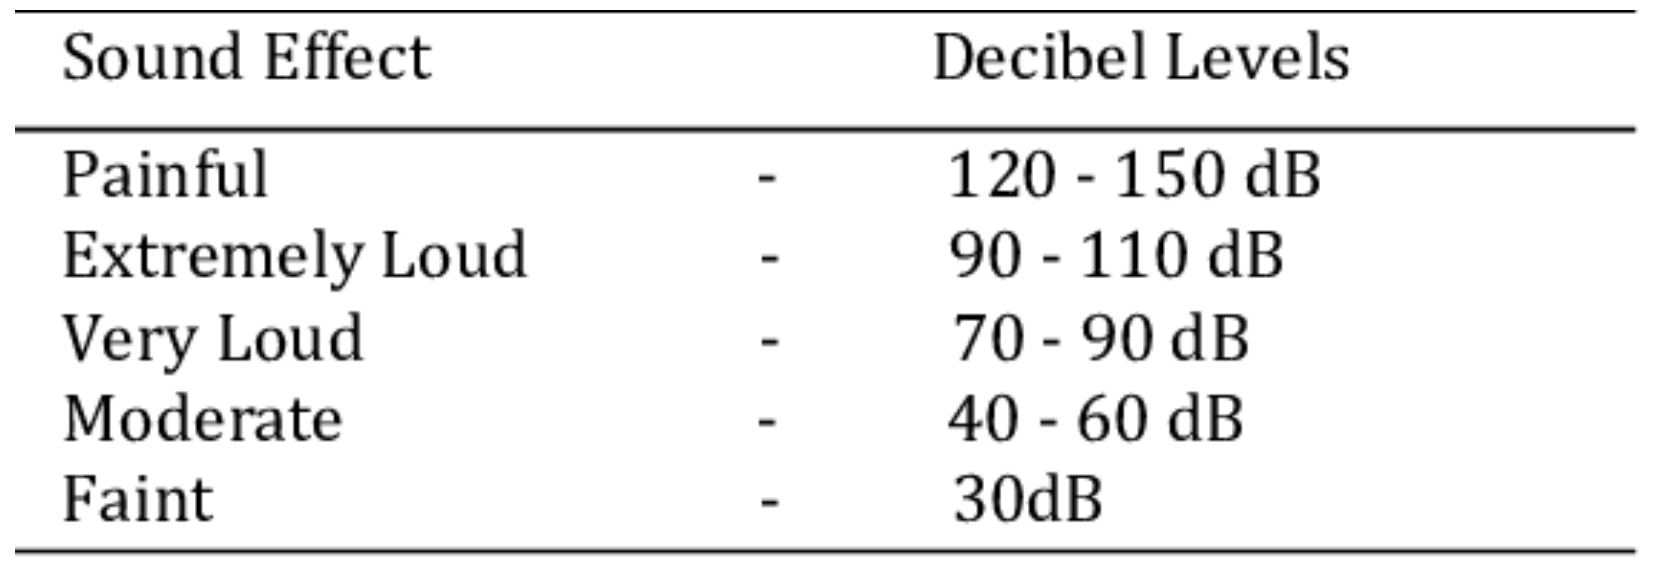
\includegraphics[width=0.85\textwidth]{soundChart} \\[12pt]
	\cite{sound}
\end{center}

\subsubsection{Interferences in Sound}
Sound waves can vary greatly in frequency, ranging from lower pitches around 20 Hz up to super sonic sounds at 60 kHz. The frequency at which a sound is produced greatly influences how it is affected by the environment through which it travels. High frequency sounds have a tendency to be absorbed by obstructions in the environment, such as leaves, and obstructions by nature limit the range at which high frequency sounds can travel. In contrast lower frequency sounds have more ``flexibility'' and can move through more obstructions in an environment, allowing them to travel much further than high frequency sounds. This leads to very different sound profiles depending on the geographical location in which observations take place.\par
We use tools called spectrograms in order to visualize these discrepancies within geographical locations. It is important that, when conducting research in soundscape ecology, we keep in mind how the physical environment will block the more delicate higher frequency sounds from the observer. This is usually counteracted by using multiple recording devices placed in equidistant patterns that cover the area of interest. Using this technique allows recording devices in better positions to pick up on sounds that obstructed devices might miss.

\subsubsection{Spectrograms}
\begin{center}
  \includegraphics[width=0.85\textwidth]{spectrogram} \\[12pt]
\end{center}
It is not uncommon in soundscape ecology to see images as the one pictured above. These graphics are called spectrograms, and they allow soundscape ecologists to visualize frequencies over time. A spectrogram is read from left to right following the passage of time. Moving up the $y$-axis shows a linear increase in frequency and a corresponding increase in pitch. The darker colors show the intensity of a sound at that particular sound range. The lighter the color the softer the sound at that frequency is. The colors depend on what spectrogram one is looking at, but there should be a legend on the side describing the nuances of each specific graph. It is common for some indices (more information in the Soundscape Ecology Indices section) to divide the spectrogram into bands of frequencies. These bands are then compared by ratios to pull out the diversity of a certain sound clip.\par
The mechanism by which complex sound waves are turned into bands of frequency is central to how soundscape ecology is conducted, and so it is beneficial to have at least a basic understanding of the process. At the heart of it is the Fourier transform.\par
When we have a complicated wave created by many simple notes (simple meaning single frequency), what we experience is the addition of the two waves over a period of time. If one wave is in a descending crest while the other is ascending, then the addition is destructive. On the other hand, if both waves are cresting at the same point the interference is said to be constructive. The addition of these two waves destroys the sinusoidal nature and creates a brand new wave type. This new wave has no single frequency and thus cannot be easily displayed onto a spectrogram. This is where the Fourier transform comes into play.\par
To begin our transform we start by mapping the wave function from Cartesian coordinates to polar coordinates, as shown below.
\begin{center}
  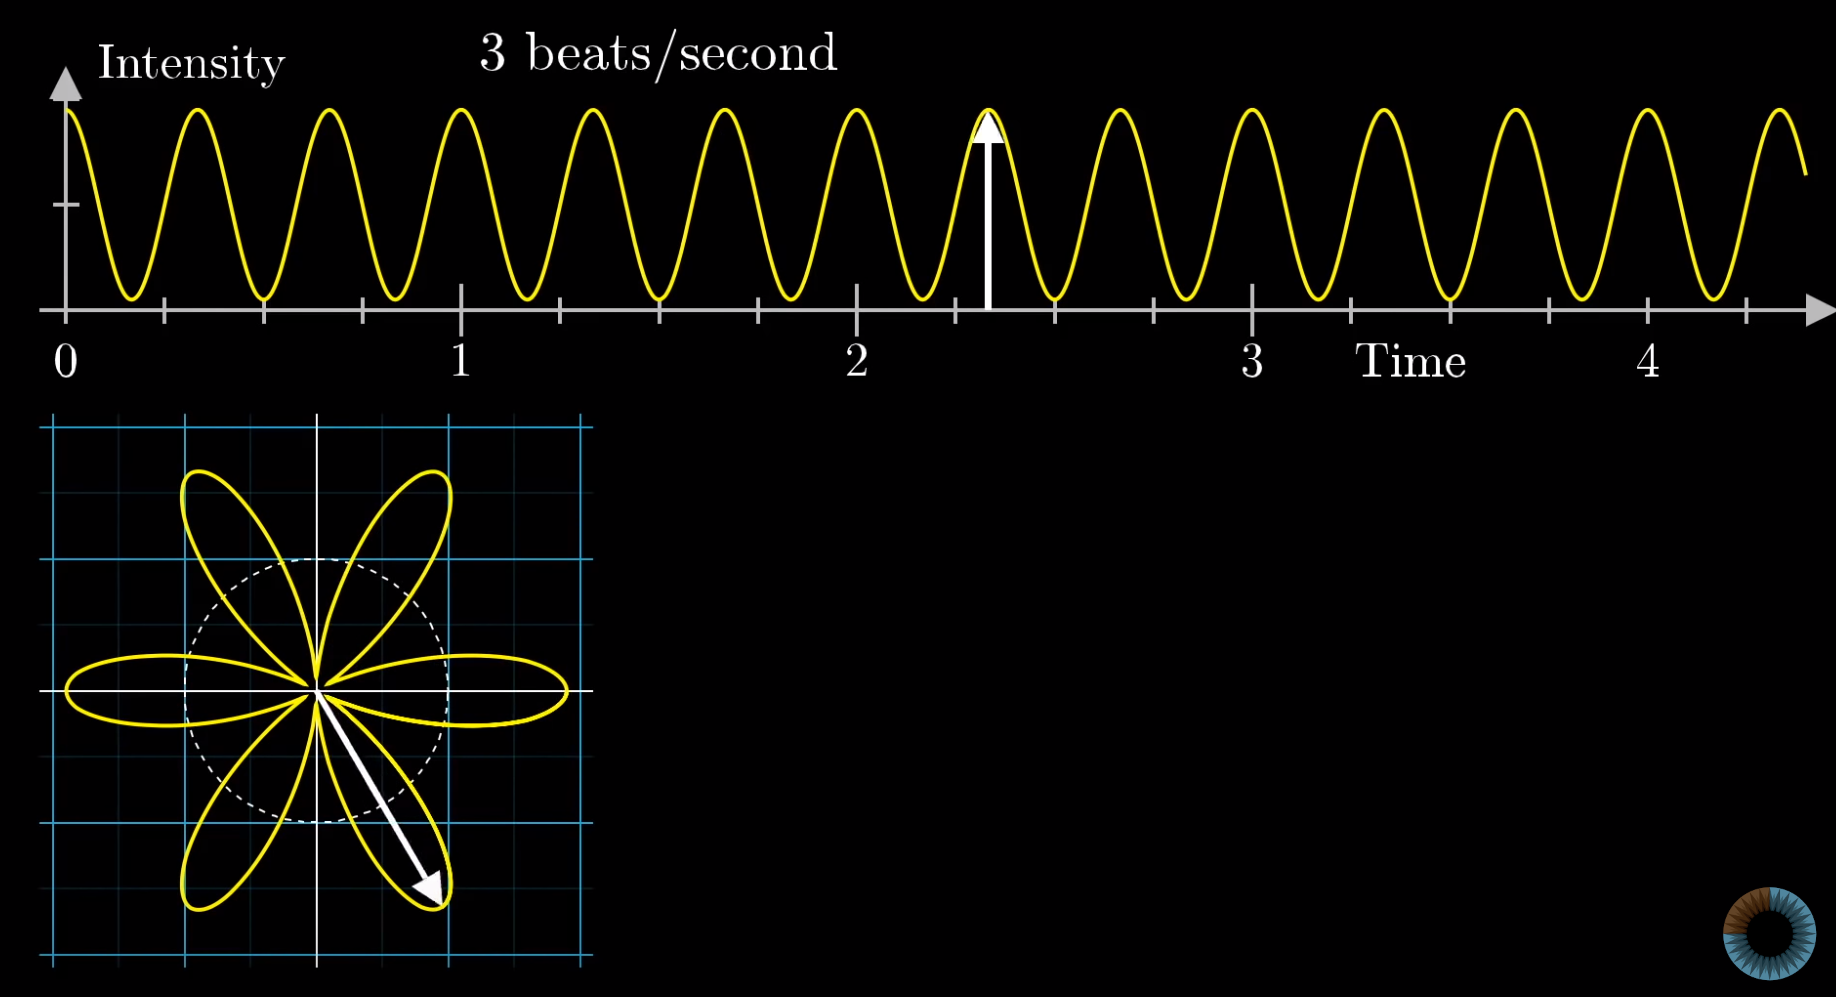
\includegraphics[width=0.85\textwidth]{polar} \\[12pt]
\end{center} \cite{bluebrown}
In the above example, the wave is plotted on the polar axis at the rate of 0.5 cycles per second. This rate can be changed, and changing it will effect how the polar coordinate graph will appear. The trick here is that if the rate at which you plot the wave onto the polar axis coincides exactly with the frequency of the original wave then the ``center of mass'' of the polar graph shifts outwards. This shift represents the intensity of a sound at that frequency. Not only can this change in the center of mass tell which frequency tones make up the original complicated wave, but it can also tell the intensity of specific frequencies within that wave. Using this, it is possible to directly map the original wave to a spectrogram. Using the $x$ position of the center of mass of the polar coordinate graph to show the intensity of a frequency, choosing the frequency is as simple as changing the cycles per second at which the graph drawn, 3 cycles per second being 3 Hz, 10 cycles per second being 10 Hz, and so on.
\begin{center}
  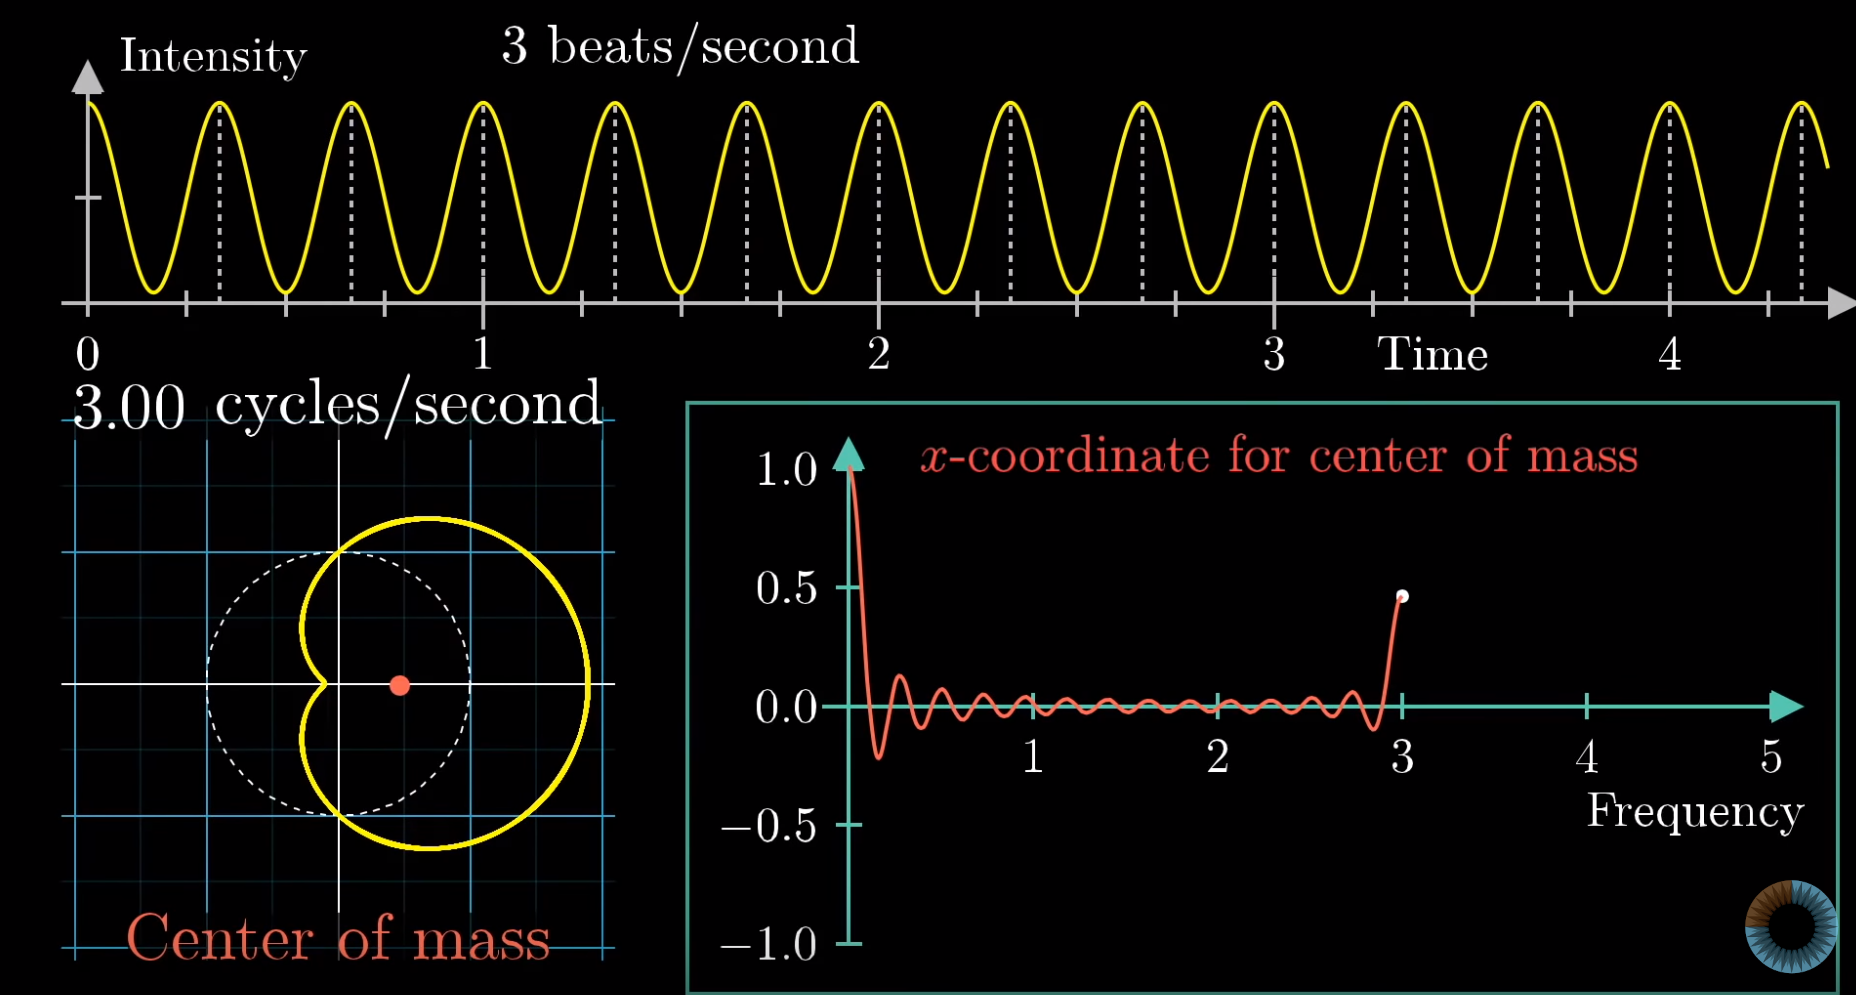
\includegraphics[width=0.85\textwidth]{centerofmass} \\
\end{center}
\begin{center}
  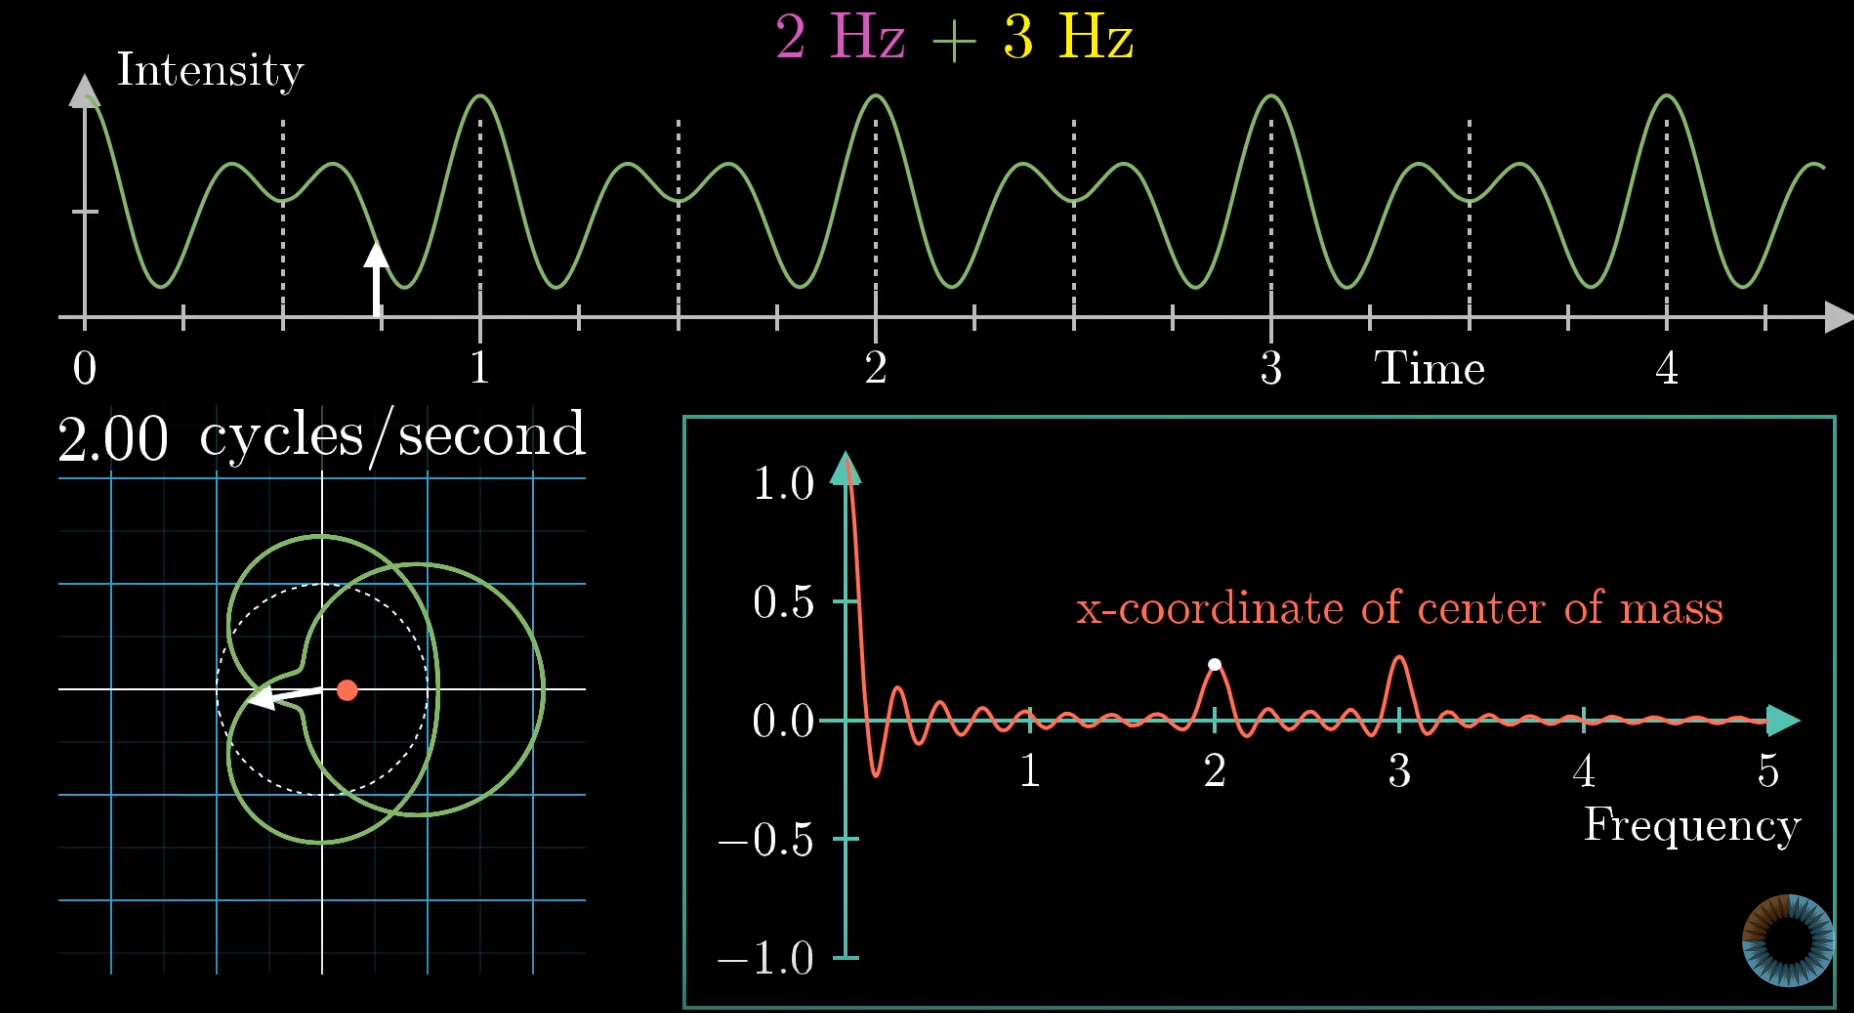
\includegraphics[width=0.85\textwidth]{shiftedcenter} \\[12pt]
  \cite{bluebrown}
\end{center}
This intuitive idea can then be boiled down to a single equation, which comprises of the integral over the initial wave function with Euler\textquotesingle s number to take into account the cyclical nature of the function. The equation is as follows \cite{bluebrown}:
\begin{equation}
  \int_{t_1}^{t_2} g(t)e^{-2\pi i f t} dt
\end{equation} \\[\eqnspace]
